\documentclass[convert={outfile=neo_ios_and_tools.svg}]{standalone}%
\usepackage{standalone}
\usepackage[T1]{fontenc}%
\usepackage[utf8]{inputenc}%
\usepackage{lmodern}%
\usepackage{textcomp}%
\usepackage[usenames,dvipsnames]{xcolor}
% \usepackage[margin=2cm]{geometry}
\usepackage{tikz}%
\usetikzlibrary{fit, fadings, shapes, backgrounds, arrows.meta, positioning,calc}%
%
%
%
\begin{document}%
\begin{tikzpicture}
\tikzstyle{io}=[rectangle,rounded corners,text centered,align=center,fill=blue!30,inner sep=7pt]
\tikzstyle{writable}=[fill=blue!50]
\tikzstyle{rawio}=[io, draw=black!80!blue, line width=1pt]
\tikzstyle{software}=[rectangle, rounded corners, text centered, align=center,fill=Mahogany!30, inner sep=7pt, draw=Mahogany, line width=2pt]
\tikzstyle{withicon}=[rectangle split, rectangle split draw splits=false, rectangle split parts=2]
\tikzstyle{title}=[font=\huge]
\tikzstyle{group}=[rectangle, inner sep=20pt, path fading = fade out, fill=gray!60]
\tikzstyle{uses}=[line width=12pt,-stealth]

% IO nodes as generated by extract_neo_ios.py
\node[io] (box0) at (0.0,0.0) {AlphaOmega};%
\node[io, writable] (box1) at (3.0,0.0) {AsciiSignal};%
\node[io, writable] (box2) at (6.0,0.0) {AsciiSpikeTrain};%
\node[rawio] (box3) at (9.0,0.0) {Axograph};%
\node[rawio] (box4) at (12.0,0.0) {Axon};%
\node[rawio] (box5) at (0.0,-2.0) {BCI2000};%
\node[rawio] (box6) at (3.0,-2.0) {Blackrock};%
\node[io] (box7) at (6.0,-2.0) {Blackrock};% 
\node[rawio] (box8) at (9.0,-2.0) {BrainVision};%
\node[io] (box9) at (12.0,-2.0) {BrainwareDam};%
\node[io] (box10) at (0.0,-4.0) {BrainwareF32};%
\node[io] (box11) at (3.0,-4.0) {BrainwareSrc};%
\node[rawio] (box12) at (6.0,-4.0) {Elan};%
\node[io] (box13) at (9.0,-4.0) {Igor};%
\node[rawio] (box14) at (12.0,-4.0) {Intan};%
\node[io, writable] (box15) at (0.0,-6.0) {KlustaKwik};%
\node[io] (box16) at (3.0,-6.0) {Kwik};%
\node[rawio] (box17) at (6.0,-6.0) {Micromed};%
\node[io, writable] (box18) at (9.0,-6.0) {NSDF};%
\node[io] (box19) at (12.0,-6.0) {NeoHdf5};%
\node[io, writable] (box20) at (0.0,-8.0) {NeoMatlab};%
\node[io] (box21) at (3.0,-8.0) {Nest};%
\node[rawio] (box22) at (6.0,-8.0) {Neuralynx};%
\node[io] (box23) at (9.0,-8.0) {Neuralynx};%
\node[rawio] (box24) at (12.0,-8.0) {NeuroExplorer};%
\node[rawio] (box25) at (0.0,-10.0) {NeuroScope};%
\node[io] (box26) at (3.0,-10.0) {Neurosharectypes};%
\node[io, writable] (box27) at (6.0,-10.0) {Nix};%
\node[rawio] (box28) at (9.0,-10.0) {Nix};%
\node[rawio] (box29) at (12.0,-10.0) {OpenEphys};%
\node[io, writable] (box30) at (0.0,-12.0) {Pickle};%
\node[rawio] (box31) at (3.0,-12.0) {Plexon};%
\node[rawio, writable] (box32) at (6.0,-12.0) {RawBinarySignal};%
\node[rawio] (box33) at (9.0,-12.0) {RawMCS};%
\node[rawio] (box34) at (12.0,-12.0) {Spike2};%
\node[io] (box35) at (0.0,-14.0) {Stimfit};%
\node[rawio] (box36) at (3.0,-14.0) {Tdt};%
\node[rawio] (box37) at (6.0,-14.0) {WinEdr};%
\node[rawio] (box38) at (9.0,-14.0) {WinWcp};%


\tikzfading[name=fade out, inner color=transparent!0, outer color=transparent!100]

% \fill[gray,path fading=fade out, fit=(box0) (box1) (box2) (box3) (box4) (box5) (box6) (box7) (box8) (box9) (box10) (box11) (box12) (box13) (box14) (box15) (box16) (box17) (box18) (box19) (box20) (box21) (box22) (box23) (box24) (box25) (box26) (box27) (box28) (box29) (box30) (box31) (box32) (box33) (box34) (box35) (box36) (box37) (box38) (box39)] ellipse;
       
\begin{pgfonlayer}{background}
\node[rectangle, rounded corners=60pt,inner sep=20pt,  %path fading=fade out,
fit=(box0) (box1) (box2) (box3) (box4) (box5) (box6) (box7) (box8) (box9) (box10) (box11)
(box12) (box13) (box14) (box15) (box16) (box17) (box18) (box19) (box20) (box21) (box22) (box23) (box24) (box25) (box26) (box27) (box28) (box29) (box30) (box31) (box32) (box33) (box34) (box35) (box36) (box37) (box38)
] (ios) {};

\end{pgfonlayer}



\node[software, withicon, above= 5cm of ios, fill=none, draw=blue!60, fill=blue!20] (neo) {\huge\textbf{{Neo}} \nodepart{two} 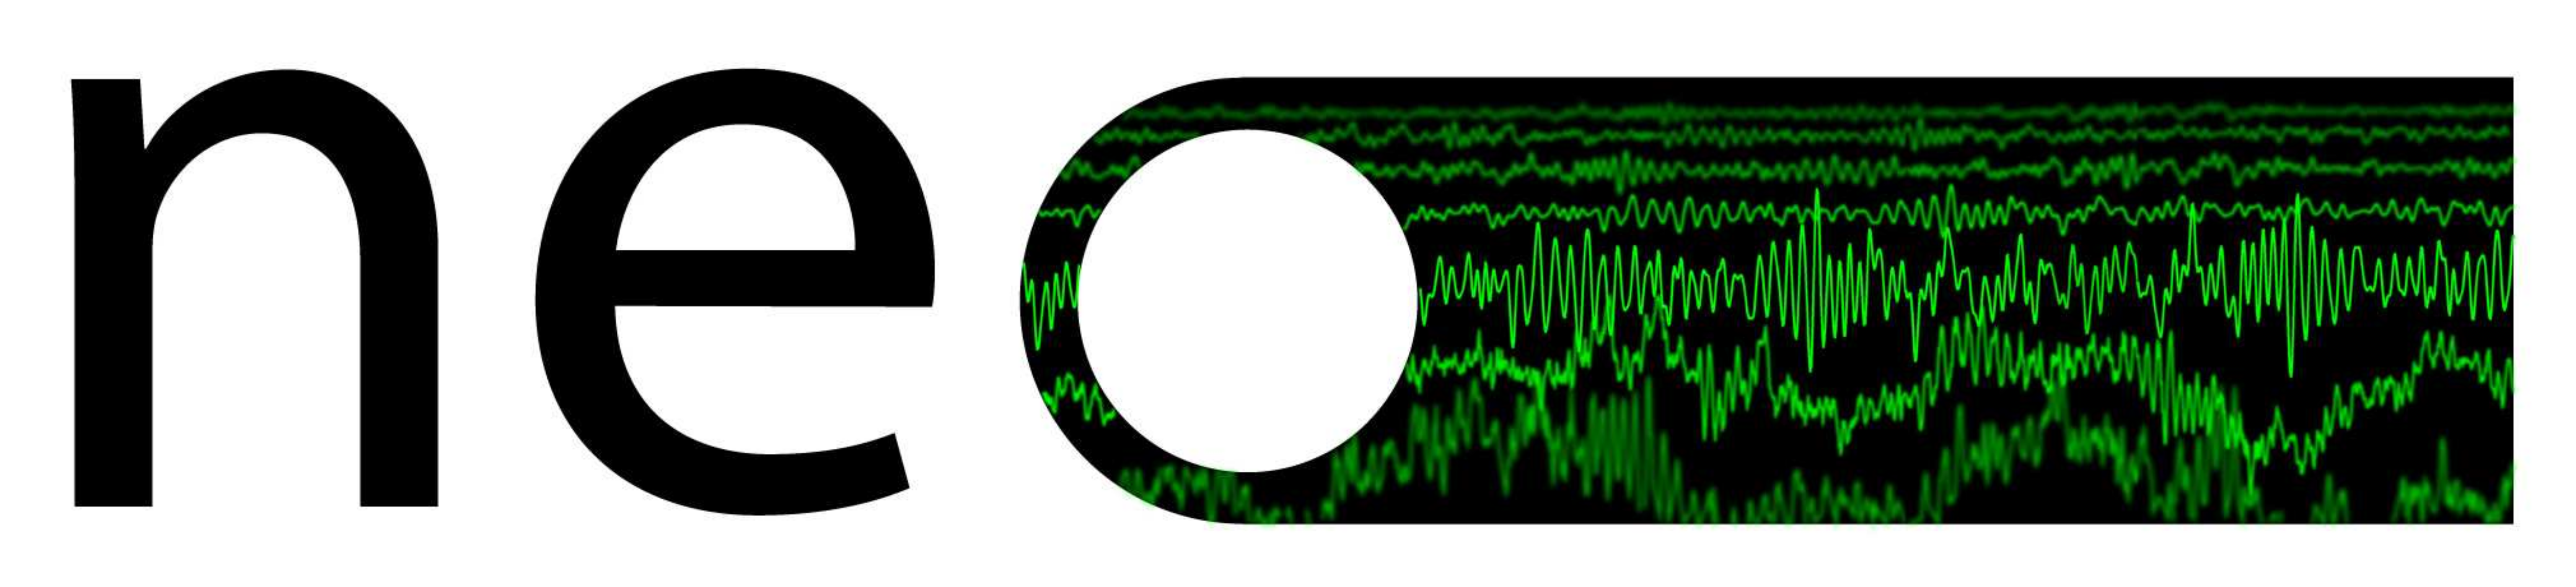
\includegraphics[width=3cm]{logos/neo}};

\begin{pgfonlayer}{background}
\fill[cyan, fill=blue!20, rounded corners=60pt] %fill opacity=0.4 
    (ios.south east) 
    to (ios.south west) 
    to (ios.north west)
    to [rounded corners=0pt] (neo.south west)
%     to [rounded corners=0pt] (neo.north west) 
%     to [rounded corners=0pt] (neo.north east)
    to [rounded corners=0pt] (neo.south east)
    to (ios.north east) 
    to cycle;
% \draw[fill=lightgray] (ios.north east)++(ios.north west)++(neo.south west) ++ (ios.north east)
\end{pgfonlayer}

\node[title, above left = 6cm of neo] (visualization) {Visualization};
\node[title, above=7cm of neo] (analysis) {Analysis};
\node[title, above right=8cm of neo] (simulation) {Simulation};
\node[title, right=4cm of neo] (databases) {Databases};


\node[software, withicon, below= of analysis] (elephant) {Elephant \nodepart{two} 
\includegraphics[width=2cm]{logos/elephant}};
\node[software, withicon, below left= of analysis] (trisdesclous) {Trisdesclous \nodepart{two} 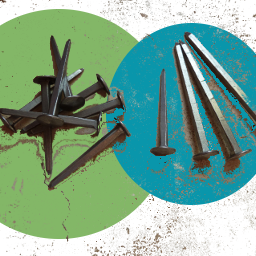
\includegraphics[width=2cm]{logos/trisdesclous}};
\node[software, withicon, below right= of analysis] (openelectrophy) {OpenElectrophy \nodepart{two} 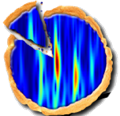
\includegraphics[width=2cm]{logos/openelectrophy}};

\node[software, withicon, below= of simulation] (pynn) {PyNN \nodepart{two} 
\includegraphics[width=1cm]{logos/pynn}};
\node[software, below=of pynn] (networkunit) {NetworkUnit};

\node[software, below= of visualization] (ephyviewer) {ephyviewer};
\node[software, withicon, below= of ephyviewer] (spykeviewer) {SpykeViewer \nodepart{two} 
\includegraphics[width=2cm]{logos/spykeviewer}};

\node[software, withicon, below= of databases] (gin) {GIN \nodepart{two} 
\includegraphics[width=2cm]{logos/gin}};

\begin{pgfonlayer}{background}
\node[group, fit=(visualization) (ephyviewer) (spykeviewer)] (vis) {};
\node[group, fit=(analysis) (trisdesclous) (elephant) (openelectrophy)] (ana) {};
\node[group, fit=(simulation) (networkunit) (pynn)] (sim) {};
\node[group, fit=(databases) (gin)] (dat) {};

\end{pgfonlayer}

\fill [gray, path fading=fade out, fit=(visualization) (ephyviewer) (spykeviewer)];


\draw[uses, bend right=15, gray] (ios) to (neo);
\draw[uses, bend right=15, lightgray] (neo) to (ios);%, transform canvas={xshift = -1cm}
\draw[uses, bend right=15, gray] (neo) to (dat);
\draw[uses, bend right=15, gray] (dat) to (neo);
\draw[uses, gray] (neo) to (vis);
\draw[uses, gray] (sim) to (neo);
\draw[uses, bend right=15, gray] (neo) to (ana);
\draw[uses, bend right=15, gray] (ana) to (neo);


\end{tikzpicture}

\end{document}
